% ----------------------------------------------------------------------------------------------------------
% Anhang
% ----------------------------------------------------------------------------------------------------------

\renewcommand\refname{Anhang}
\begin{appendix}
\chapter{Anhang}

\vspace{1em}
\begin{minipage}{\linewidth}
	\centering
	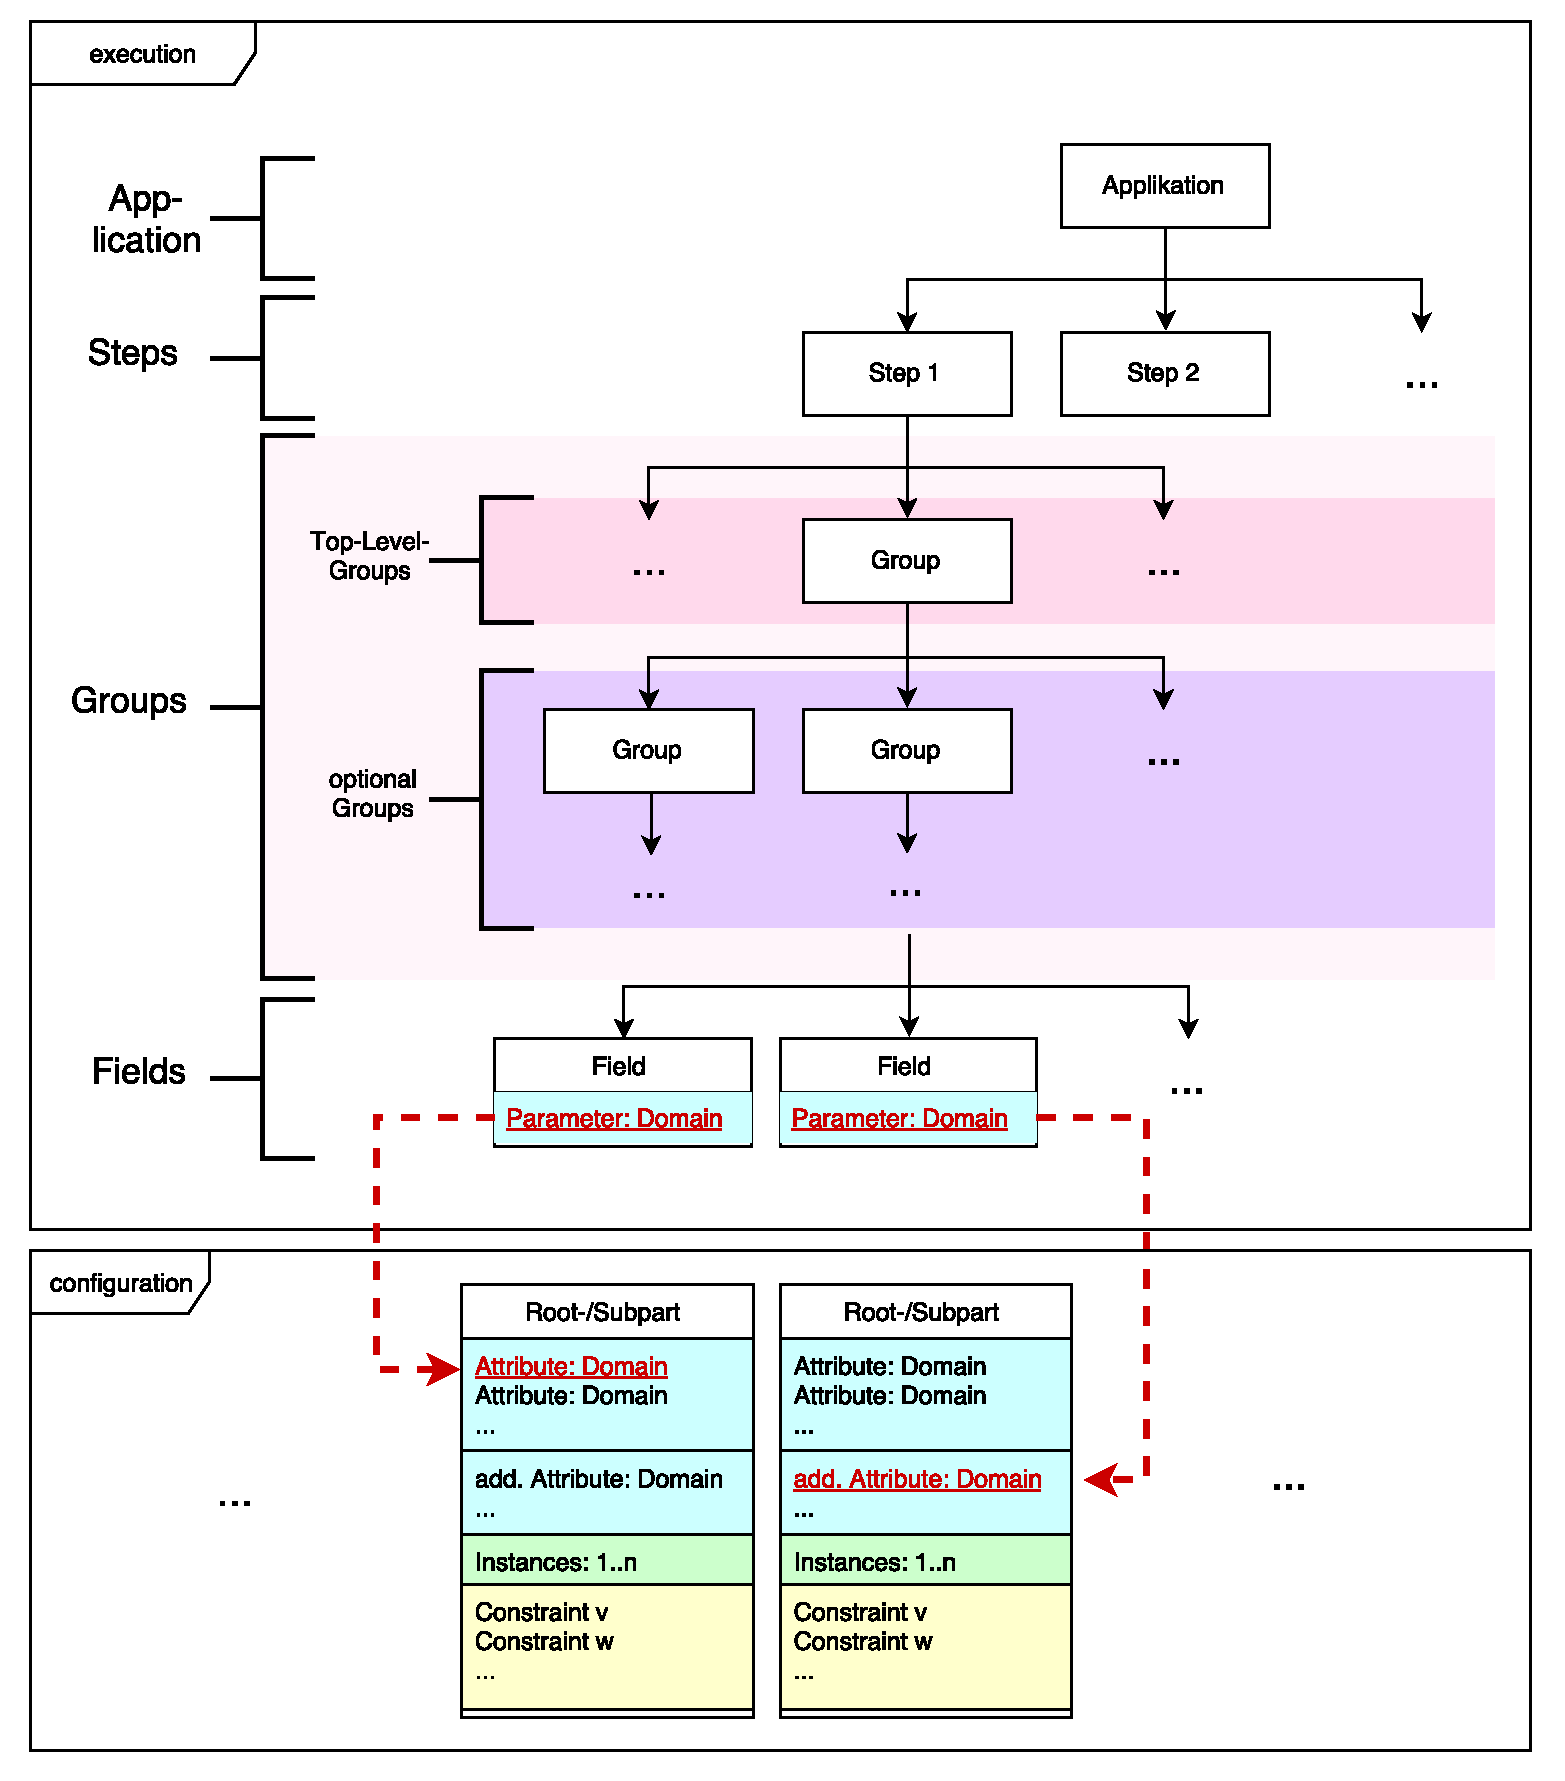
\includegraphics[width=1\linewidth]{Abbildungen/tactonModellExecution.pdf}
	\captionof{figure}[Vollständige Darstellung der generischen Execution-Struktur]{Vollständige Darstellung der generischen Execution-Struktur}
	\label{app:tactonModellExecutionLong}
\end{minipage}
\vspace{1em}

\vspace{1em}
\begin{minipage}{\linewidth}
	\centering
	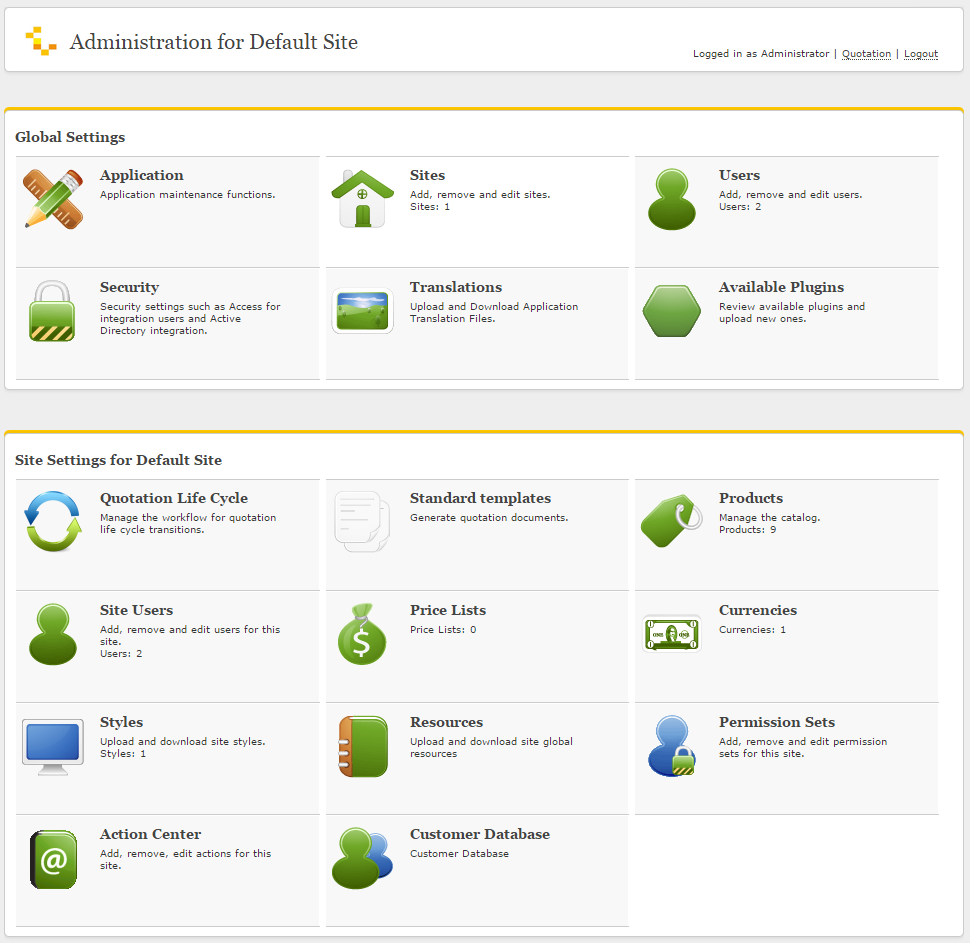
\includegraphics[width=1\linewidth]{Abbildungen/tcsiteAdministration.PNG}
	\captionof{figure}[tcsiteAdministration]{TCsite Administrationsoberfläche}
	\label{app:tcsiteAdministration}
\end{minipage}
\vspace{1em}

\vspace{1em}
\begin{minipage}{\linewidth}
	\centering
	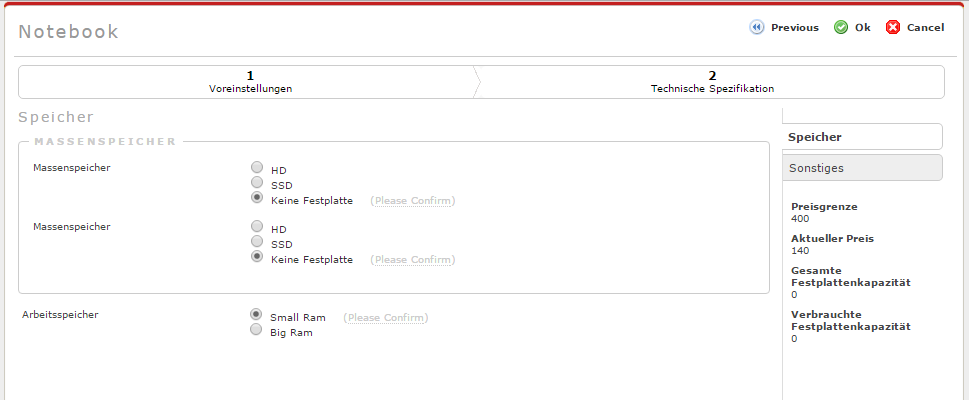
\includegraphics[width=1\linewidth]{Abbildungen/tcSiteConfigurationOptionalGroups.PNG}
	\captionof{figure}[tcSiteConfigurationOptionalGroups]{Darstellung optionaler Groups in TCsite}
	\label{app:tcSiteConfigurationOptionalGroups}
\end{minipage}
\vspace{1em}

\vspace{1em}
\begin{minipage}{\linewidth}
	\centering
	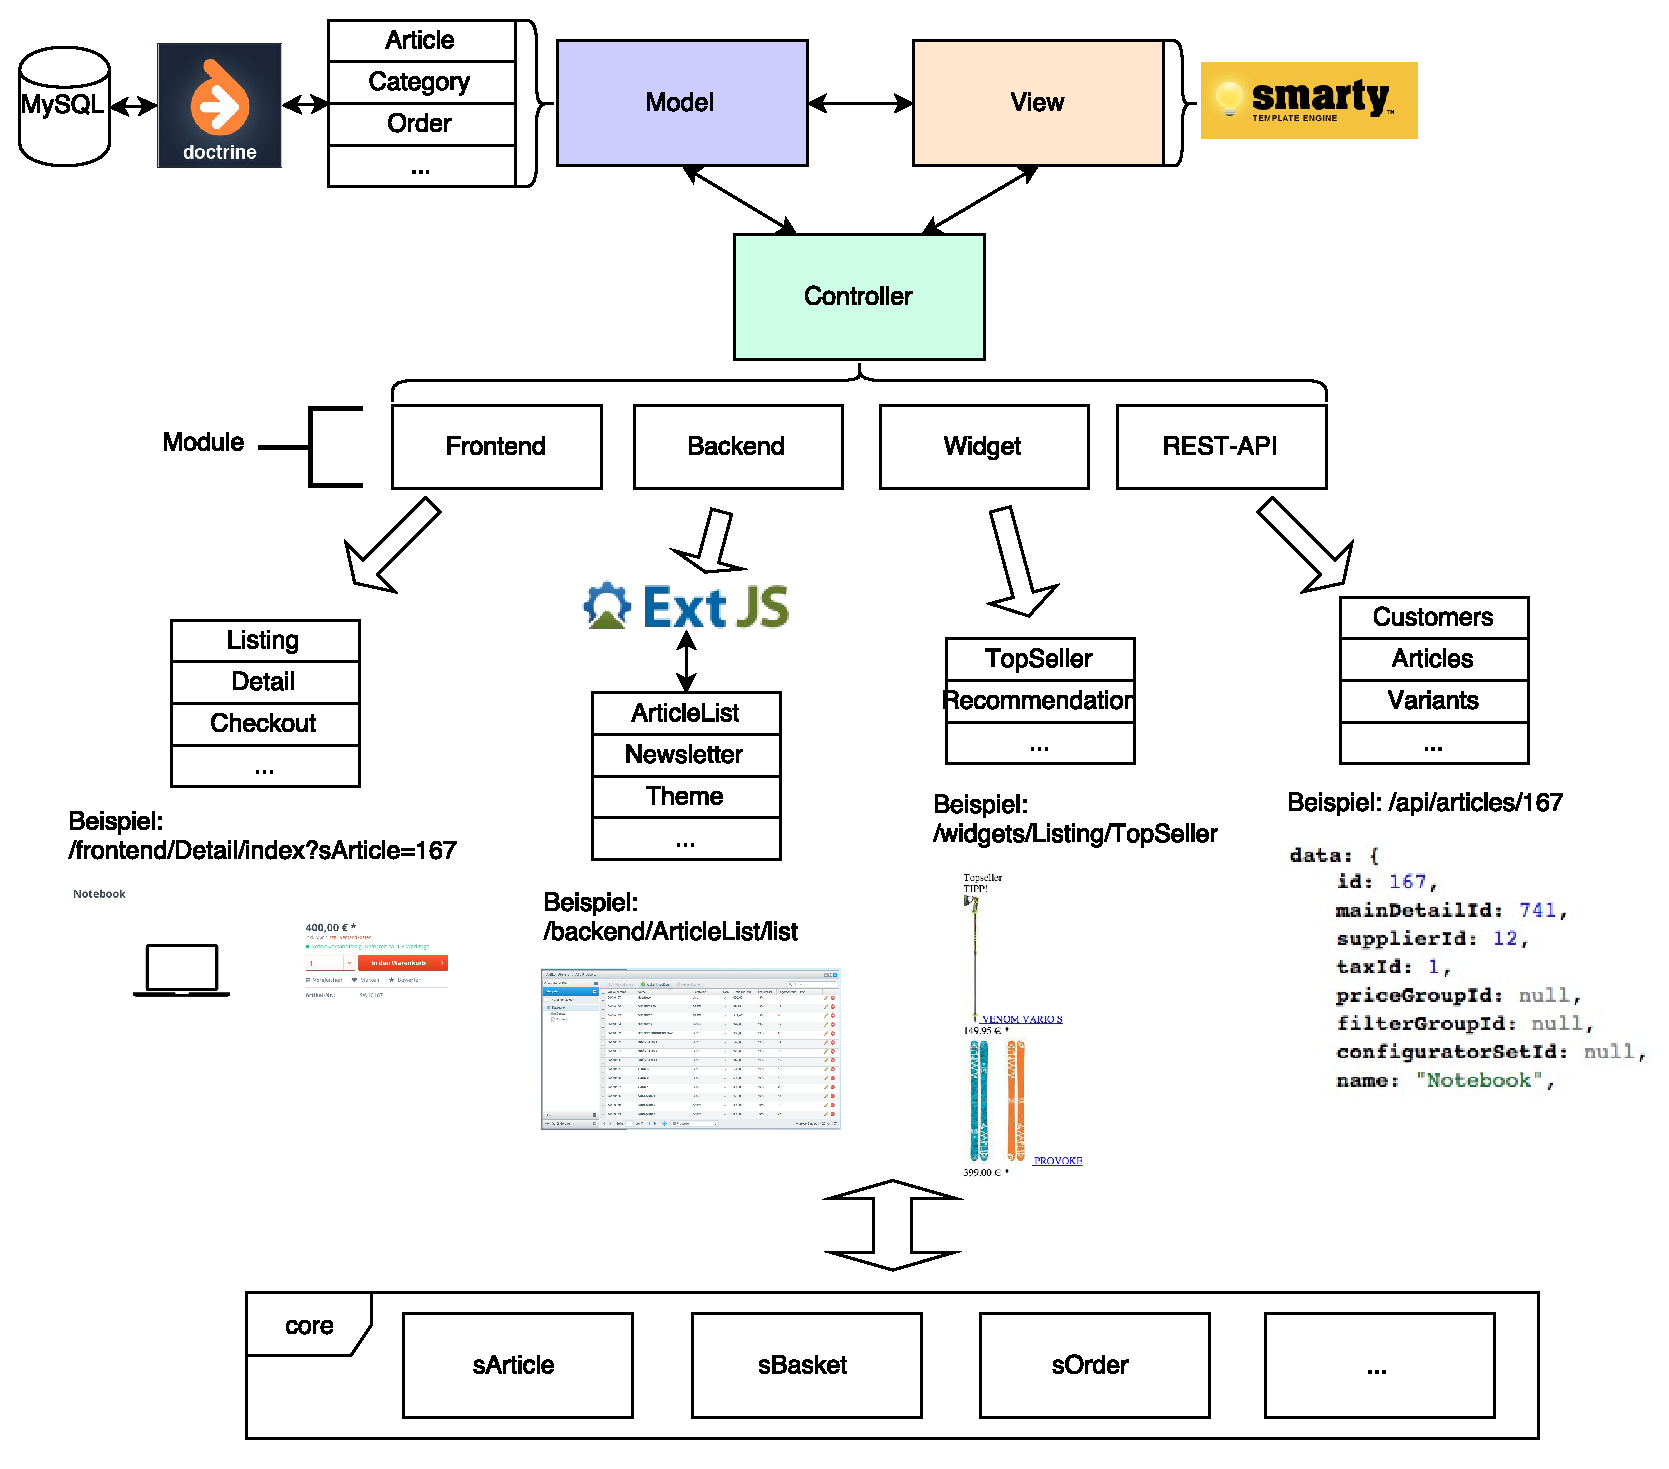
\includegraphics[width=1\linewidth]{Abbildungen/shopwareMVC.pdf}
	\captionof{figure}[vollständige High-Level-Architektur von Shopware]{vollständige Shopware High-Level-Architektur}
	\label{fig:shopwareMVCLong}
\end{minipage}
\vspace{1em}

\vspace{1em}
\begin{minipage}{\linewidth}
	\centering
	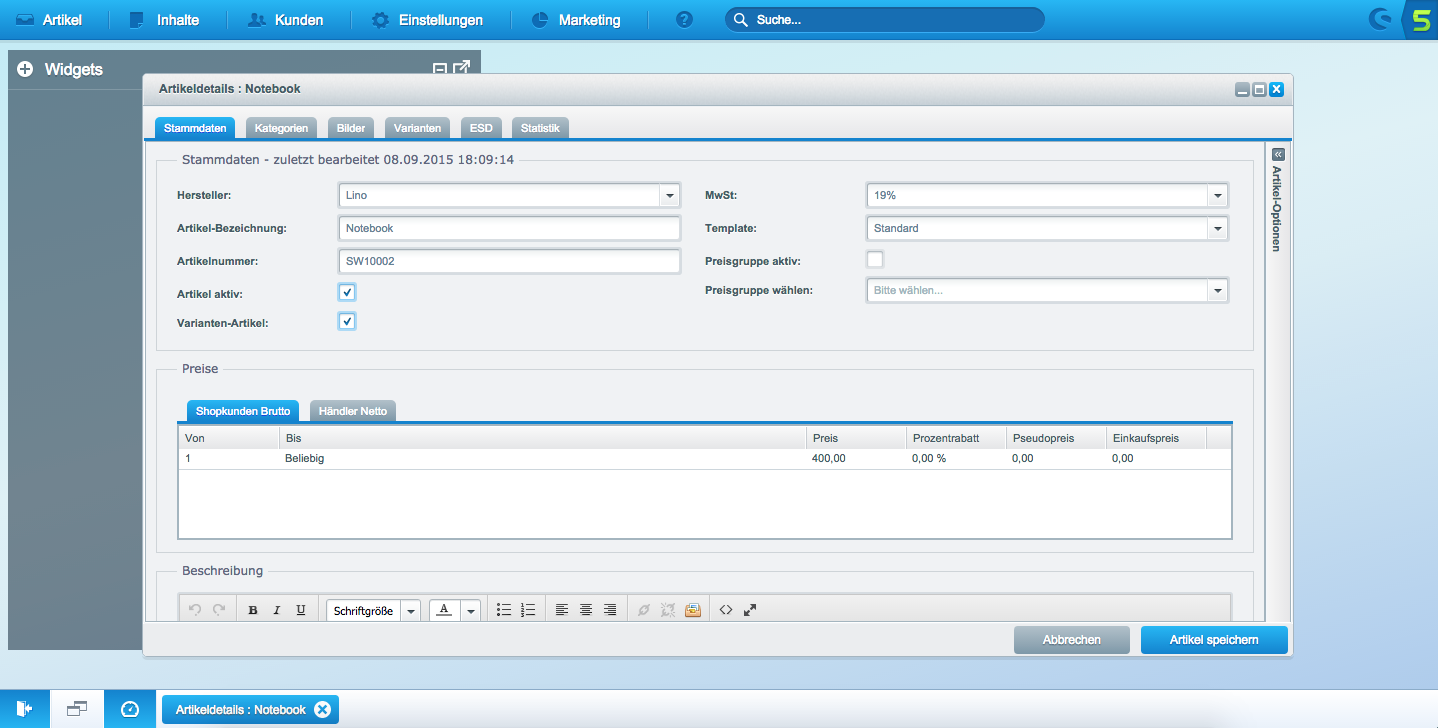
\includegraphics[width=1\linewidth]{Abbildungen/shopwareBackendArtikel.png}
	\captionof{figure}[shopwareBackendArtikel]{Anlegen eines Artikels im Backend}
	\label{app:shopwareBackendArtikel}
\end{minipage}
\vspace{1em}

\vspace{1em}
\begin{minipage}{\linewidth}
	\centering
	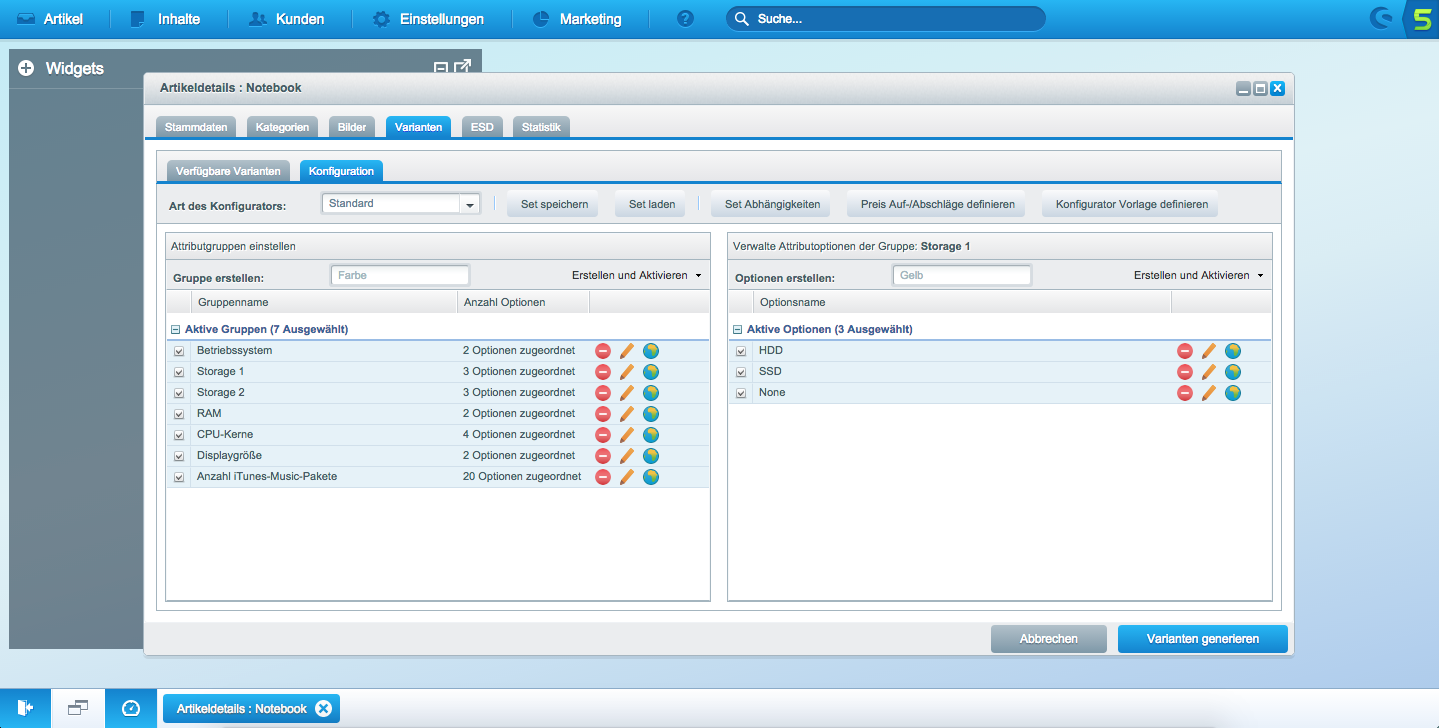
\includegraphics[width=1\linewidth]{Abbildungen/shopwareBackendArtikelVarianten.png}
	\captionof{figure}[shopwareBackendArtikelVarianten]{Generieren der Varianten im Backend}
	\label{app:shopwareBackendArtikelVarianten}
\end{minipage}
\vspace{1em}

\vspace{1em}
\begin{minipage}{\linewidth}
	\centering
	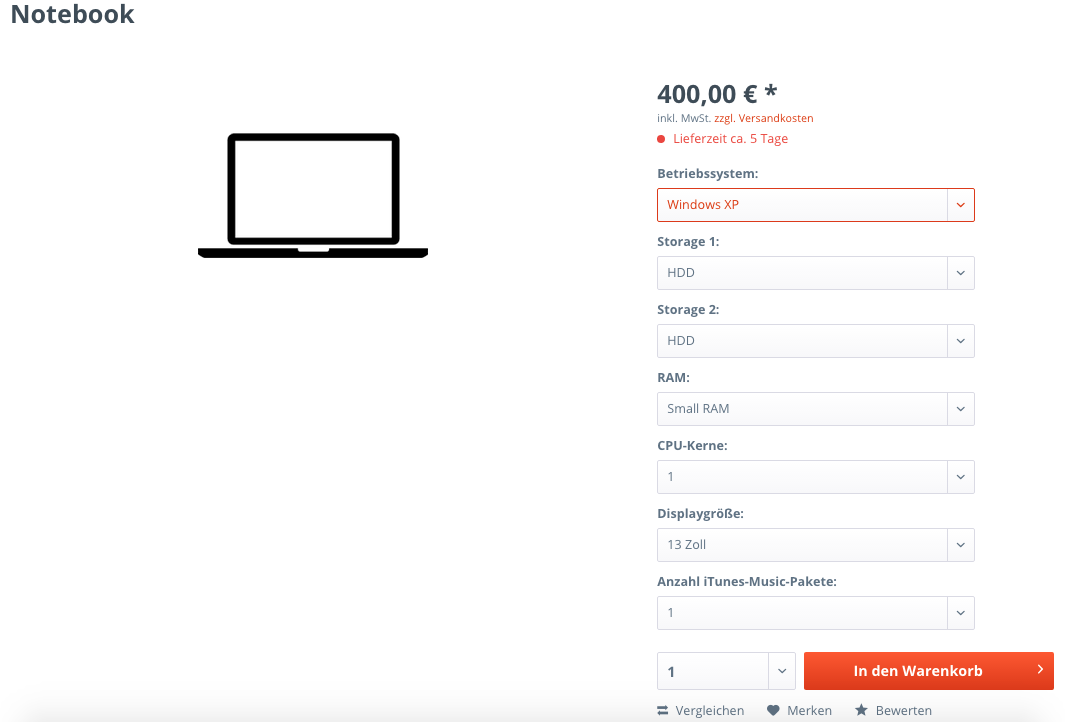
\includegraphics[width=1\linewidth]{Abbildungen/shopwareNotebookDetail.png}
	\captionof{figure}[shopwareNotebookDetail]{Detailansicht eines konfigurierbaren Notebooks in shopware.}
	\label{app:shopwareNotebookDetail}
\end{minipage}
\vspace{1em}

\vspace{1em}
\begin{minipage}{\linewidth}
	\centering
	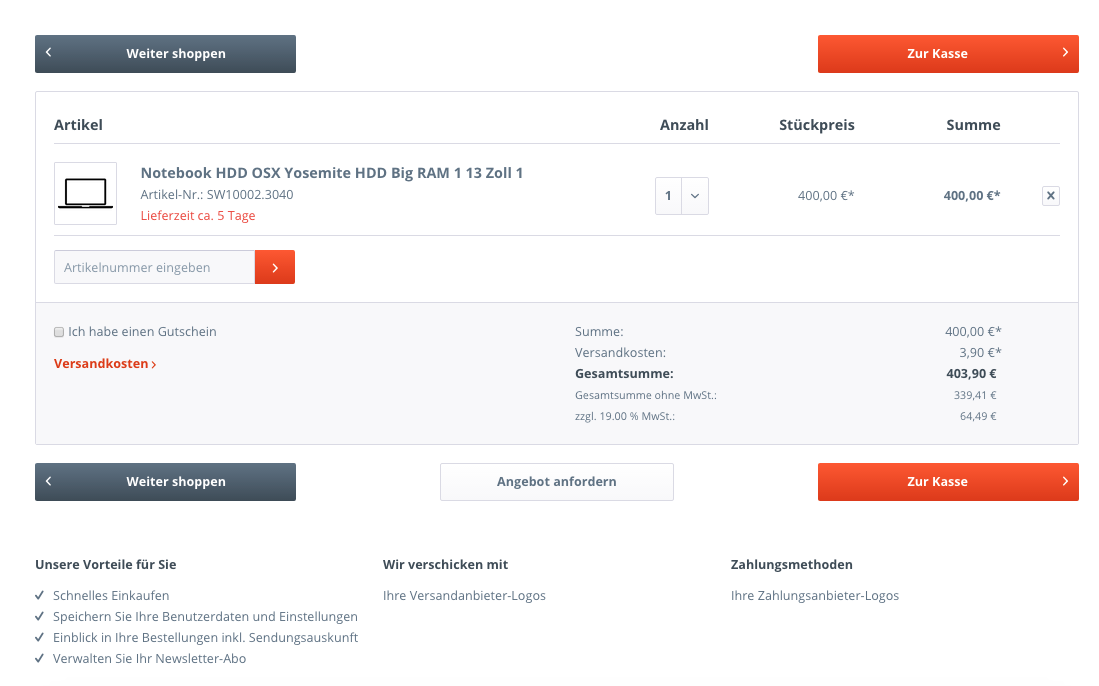
\includegraphics[width=1\linewidth]{Abbildungen/shopwareNotebookWarenkorb.png}
	\captionof{figure}[shopwareNotebookWarenkorb]{Warenkorb mit konfiguriertem Artikel.}
	\label{app:shopwareNotebookWarenkorb}
\end{minipage}
\vspace{1em}

\vspace{1em}
\begin{minipage}{\linewidth}
	\centering
	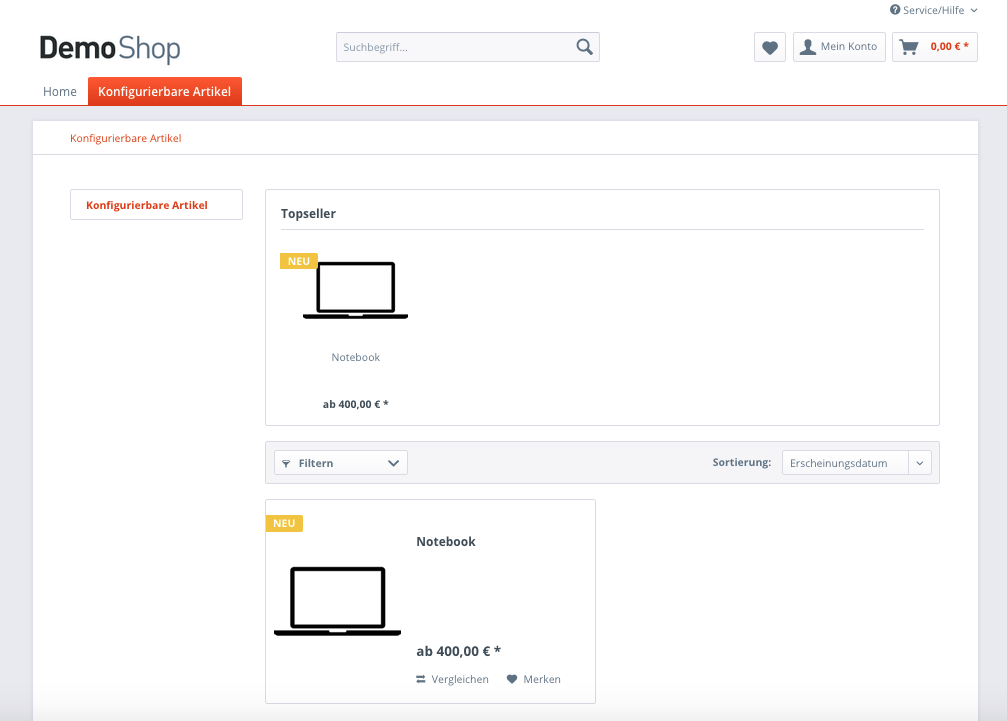
\includegraphics[width=1\linewidth]{Abbildungen/shopwareArtikelListing.png}
	\captionof{figure}[Artikellisting in Shopware]{Artikellisting in Shopware}
	\label{app:shopwareArtikelListing}
\end{minipage}
\vspace{1em}

\vspace{1em}
\begin{minipage}{\linewidth}
	\centering
	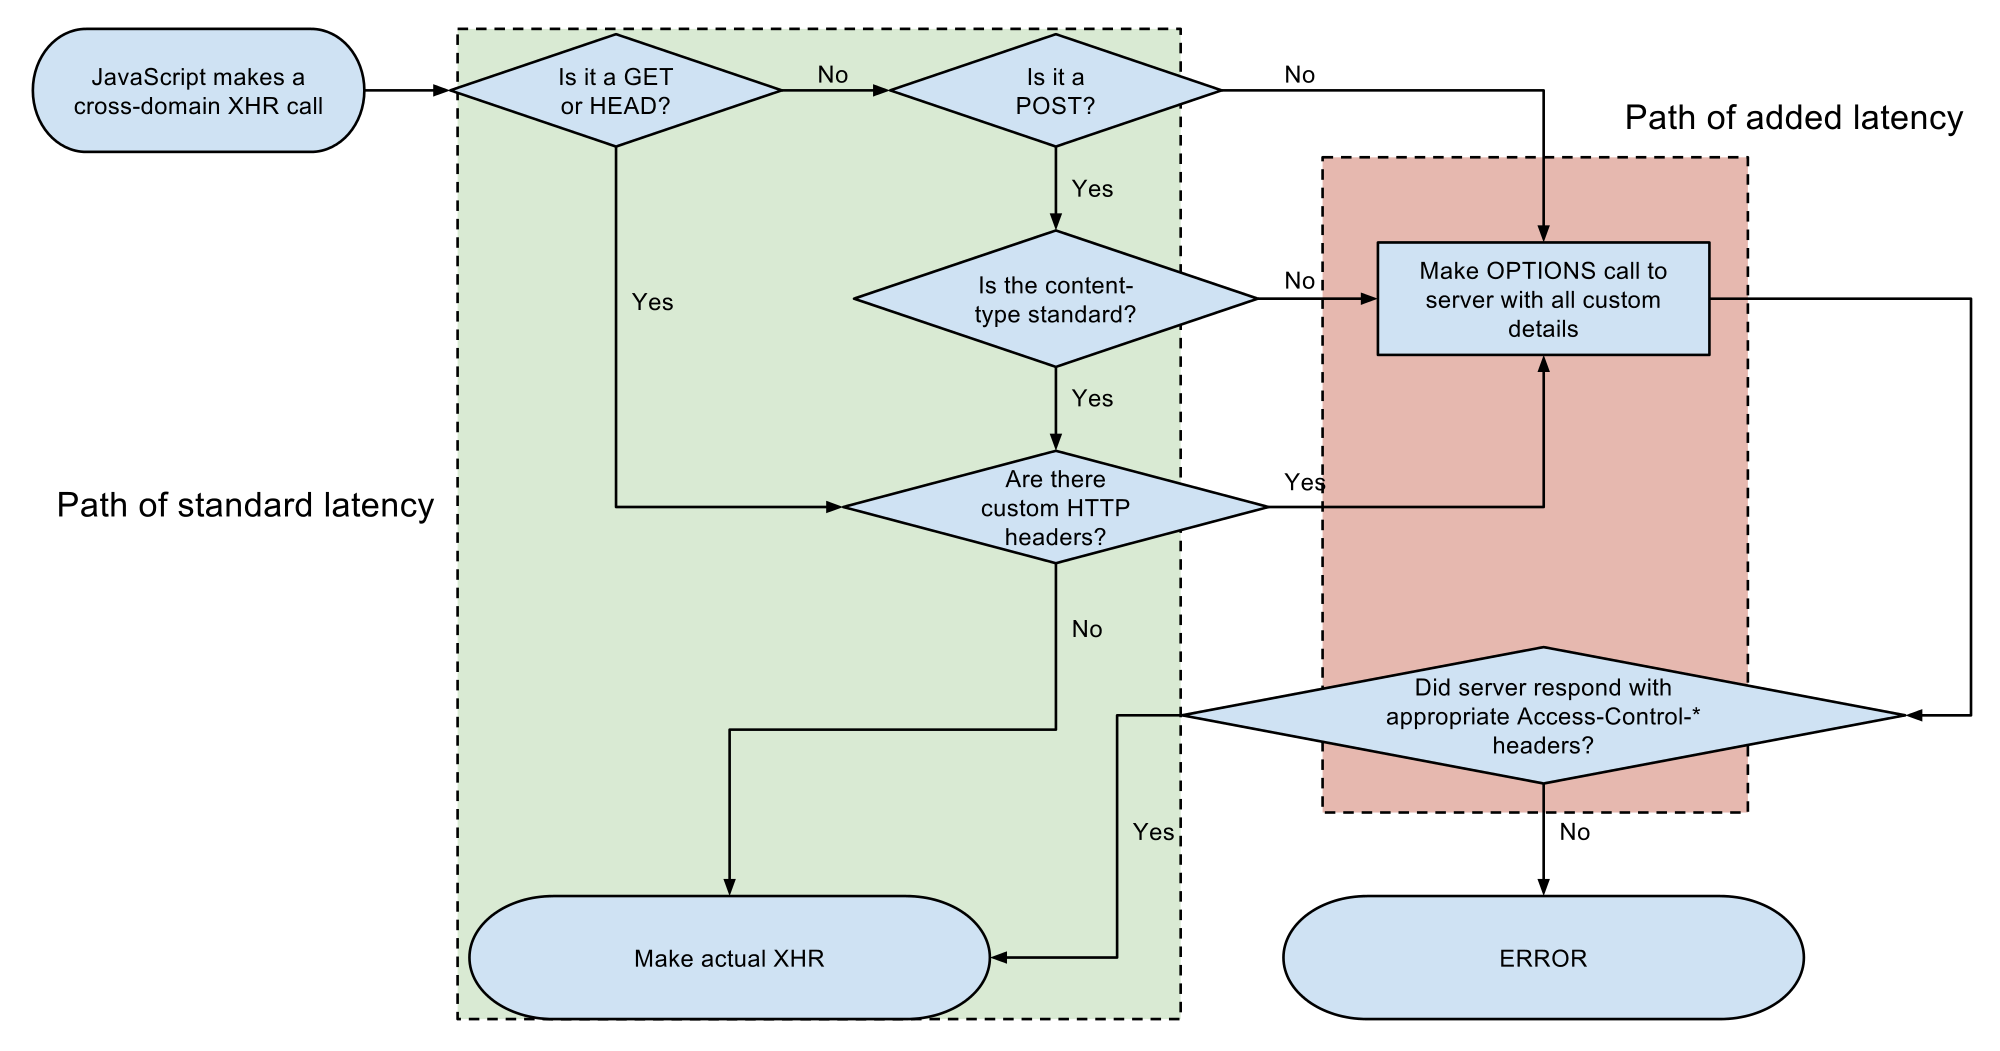
\includegraphics[width=1\linewidth]{Abbildungen/mozillaCORS.png}
	\captionof{figure}[mozillaCORS]{CORS-Flowchart.}
	\label{app:mozillaCORS}
\end{minipage}
\vspace{1em}

\vspace{1em}
\begin{minipage}{\linewidth}
	\centering
	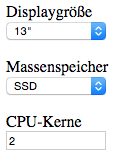
\includegraphics[width=0.2\linewidth]{Abbildungen/provisorischeEingabemaske.png}
	\captionof{figure}[provisorische Eingabemaske]{provisorische Eingabemaske}
	\label{app:provisorischeEingabemaske}
\end{minipage}
\vspace{1em}

\vspace{1em}
\begin{minipage}{\linewidth}
	\centering
	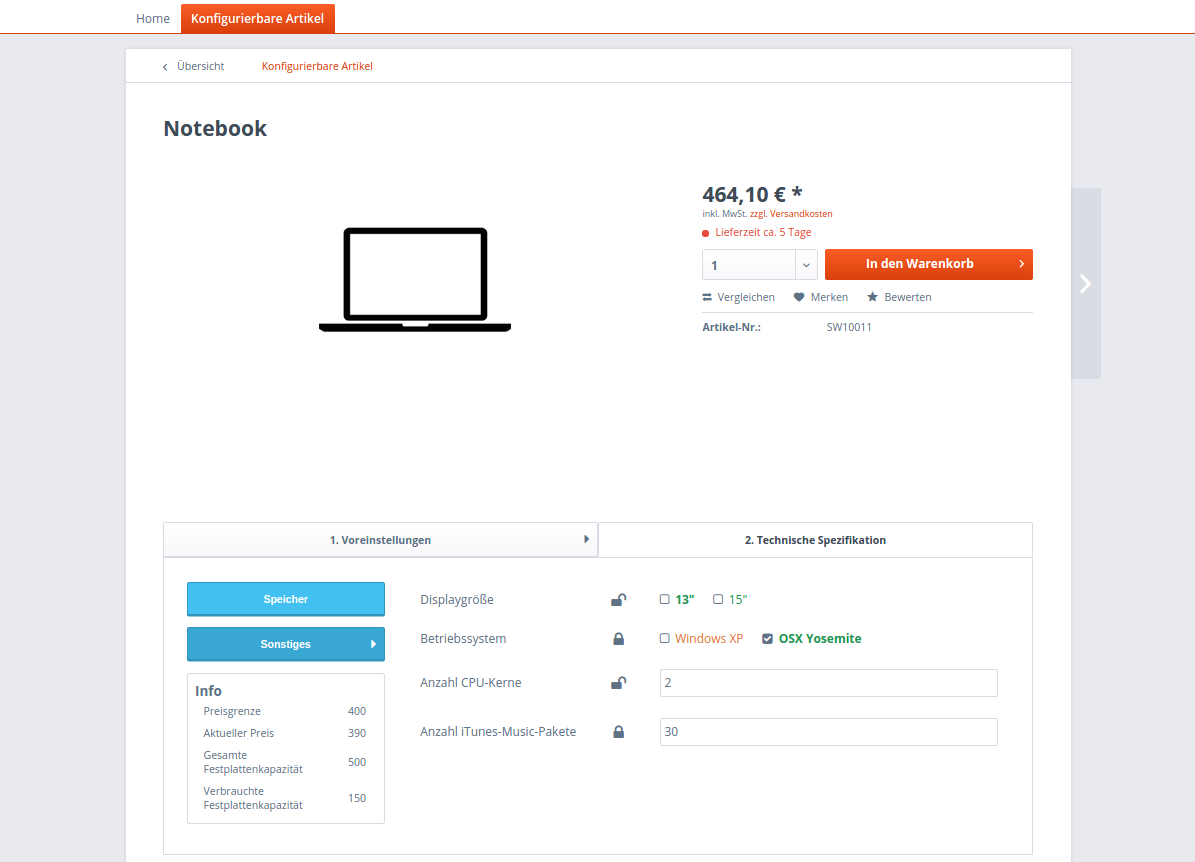
\includegraphics[width=1\linewidth]{Abbildungen/finaleKonfigurationsOberflaeche.PNG}
	\captionof{figure}[finale Konfigurationsoberfläche in Shopware]{finale Konfigurationsoberfläche in Shopware}
	\label{app:finaleKonfigurationsOberflaeche}
\end{minipage}
\vspace{1em}

\end{appendix}